\documentclass[12pt,a4paper]{article}
\usepackage[utf8]{inputenc}
\usepackage{graphicx}
\usepackage[a4paper,includeall,bindingoffset=0cm,margin=1cm,
            marginparsep=0cm,marginparwidth=0cm,top=1cm,bottom=1cm,left=2cm]{geometry}

\usepackage{avant} % Use the Avantgarde font for headings
\usepackage{graphicx} % Required for including pictures
\graphicspath{{figures/}{../figures/}}

\usepackage{tikz} % Required for drawing custom shapes
\usetikzlibrary{arrows,positioning,shapes.geometric}

\usepackage{xcolor} % rowcolor
% \usepackage{xcolor} % Required for specifying colors by name
% \definecolor{ocre}{RGB}{243,102,25} % Define the orange color used for highlighting throughout the book
\definecolor{ocre}{RGB}{25,102,243} % blue
\definecolor{tblue}{RGB}{25,102,243} % blue
\definecolor{tbrown}{rgb}{0.8, 0.0, 0.0} % brown
% \definecolor{tpink}{rgb}{1.0, 0.13, 0.32} % pink
\definecolor{tpink}{rgb}{0.93, 0.23, 0.51} 
\definecolor{tyellow}{rgb}{1.0, 0.75, 0.0} % yellow
\definecolor{tgreen}{rgb}{0.0, 0.5, 0.0} % green

\begin{document}

\begin{titlepage}

\thispagestyle{empty}

\tikzset{
  chaptertitle/.style={
    line width = 2pt ,
    rounded corners = 15pt ,
    draw = tblue,
    fill = tblue!10 ,
    fill opacity = 1 ,
    inner sep = 18pt ,
    text height = 15pt,
    text = tblue,
    node font = \Large\sffamily\bfseries ,
    text width = \paperwidth - 5.5cm, % width of the text
    align = left,
  },
  tfont/.style={
  	node font = \normalsize\sffamily\itshape,
  },
  tfont2/.style={
  	node font = \Large\sffamily\bfseries,
  }
}


\begin{tikzpicture}[remember picture]
\node[inner sep=0pt] (whitehead) at (0,0)
    {
\includegraphics[height=2cm]{laga}};
\node[inner sep=0pt] (whitehead) at (7cm,0)
    {
\includegraphics[width=7.75cm]{paris13}};
%			{
\includegraphics[width=7.5cm]{up13}};
\node[inner sep=0pt] (russell) at (14cm,0)
    {
\includegraphics[width=4.5cm]{galilee}};
\end{tikzpicture}

\bigskip

\begin{center}
\sffamily
École Doctorale 146\bigskip

{\Large\color{black!80} \textbf{THESIS}} \medskip

submitted for obtaining the degree of Doctor from\medskip

{\Large\color{black!80} \textbf{Paris 13 University}}\bigskip

Specialty ``\textit{Applied Mathematics}"
\end{center}

\begin{tikzpicture}[remember picture]  
  \node at (0,0){
      \begin{tikzpicture}[remember picture,overlay]
        \node[chaptertitle] (title) at (8.5cm,-2cm){
          Finite Element Methods for nonlinear interface problems. Application to a biofilm growth model
        };
      \end{tikzpicture}
    };
  
  \node [tfont2,tgreen] (DAT) at (15cm, -4.4cm) {DINH Anh-Thi};
%  \node [tfont, left = 0cm of DAT,black!80] {présentée et soutenue publiquement par};
	\node [tfont, left = 0cm of DAT,black!80] {presented by};
\end{tikzpicture}


\begin{center}
  \begin{figure}[h]
  \begin{center}
  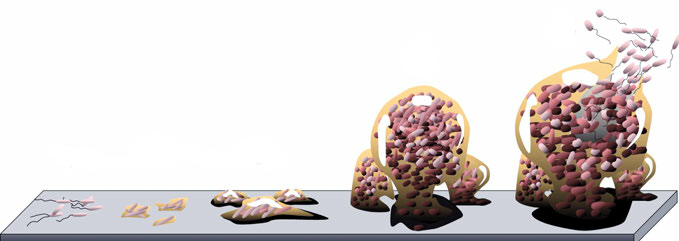
\includegraphics[width=0.8\linewidth]{biofilm}
  \end{center}
  \end{figure}
\end{center}
%
%\bigskip

\begin{center}
\normalsize\sffamily
\textbf{JURY}
%will be added later
\end{center}

\vspace{-0.2cm}

\begin{table}[hb!]
\sffamily
\centering
\begin{tabular}{lcr}
Jean-Stéphane Dhersin & Paris 13 University & Supervisor \\
Linda El Alaoui & Paris 13 University & Co-Supervisor \\
Adel Blouza & Rouen University & Co-Supervisor \\
Pascal Frey & Pierre and Marie Curie University & Reviewer \\
Yves Renard & Lyon INSA & Reviewer \\
Nicolas Vauchelet & Paris 13 University & Examiner \\
Sébastien Martin & Paris Descartes University & Examiner\\
Luís Neves de Almeida & CNRS \& Pierre and Marie Curie U. & Invited member
\end{tabular}
\end{table}

%\vspace{1cm}

\begin{center}
\sffamily
\textbf{20-12-2018} \\
Villetaneuse, France
\end{center}


\end{titlepage}

\end{document}